\documentclass[12pt,a4paper]{article}
\usepackage[utf8]{inputenc}
\usepackage{amsmath}
\usepackage{amsfonts}
\usepackage{amssymb}
\usepackage{graphicx}
\usepackage[margin=1.in]{geometry}


\author{Taylor Trabun}
%\date{A long time ago}
\title{Drone Mission Planning Software: Design Document}
\begin{document}
\maketitle

\section{Introduction}
This document provides the general design of the Drone Mission Planning Software by breaking the entire project down into several components. The current components are the physical drone, the communication system, and the graphical user interface for mission planning.

\section{Drone Design}
The drone design's major requirement that needed to be met was to achieve stable and reliable flight. 

By analyzing the drone, it was determined that its center of gravity was not directly centered on the drone, which resulted in drifting during flight. To remedy this issue, a "part holder" was designed to be mounted on the underside of the drone to hold all the motor controls, which moved the center of gravity to the center of the drone. 

\begin{figure}[h!]

  \centering
    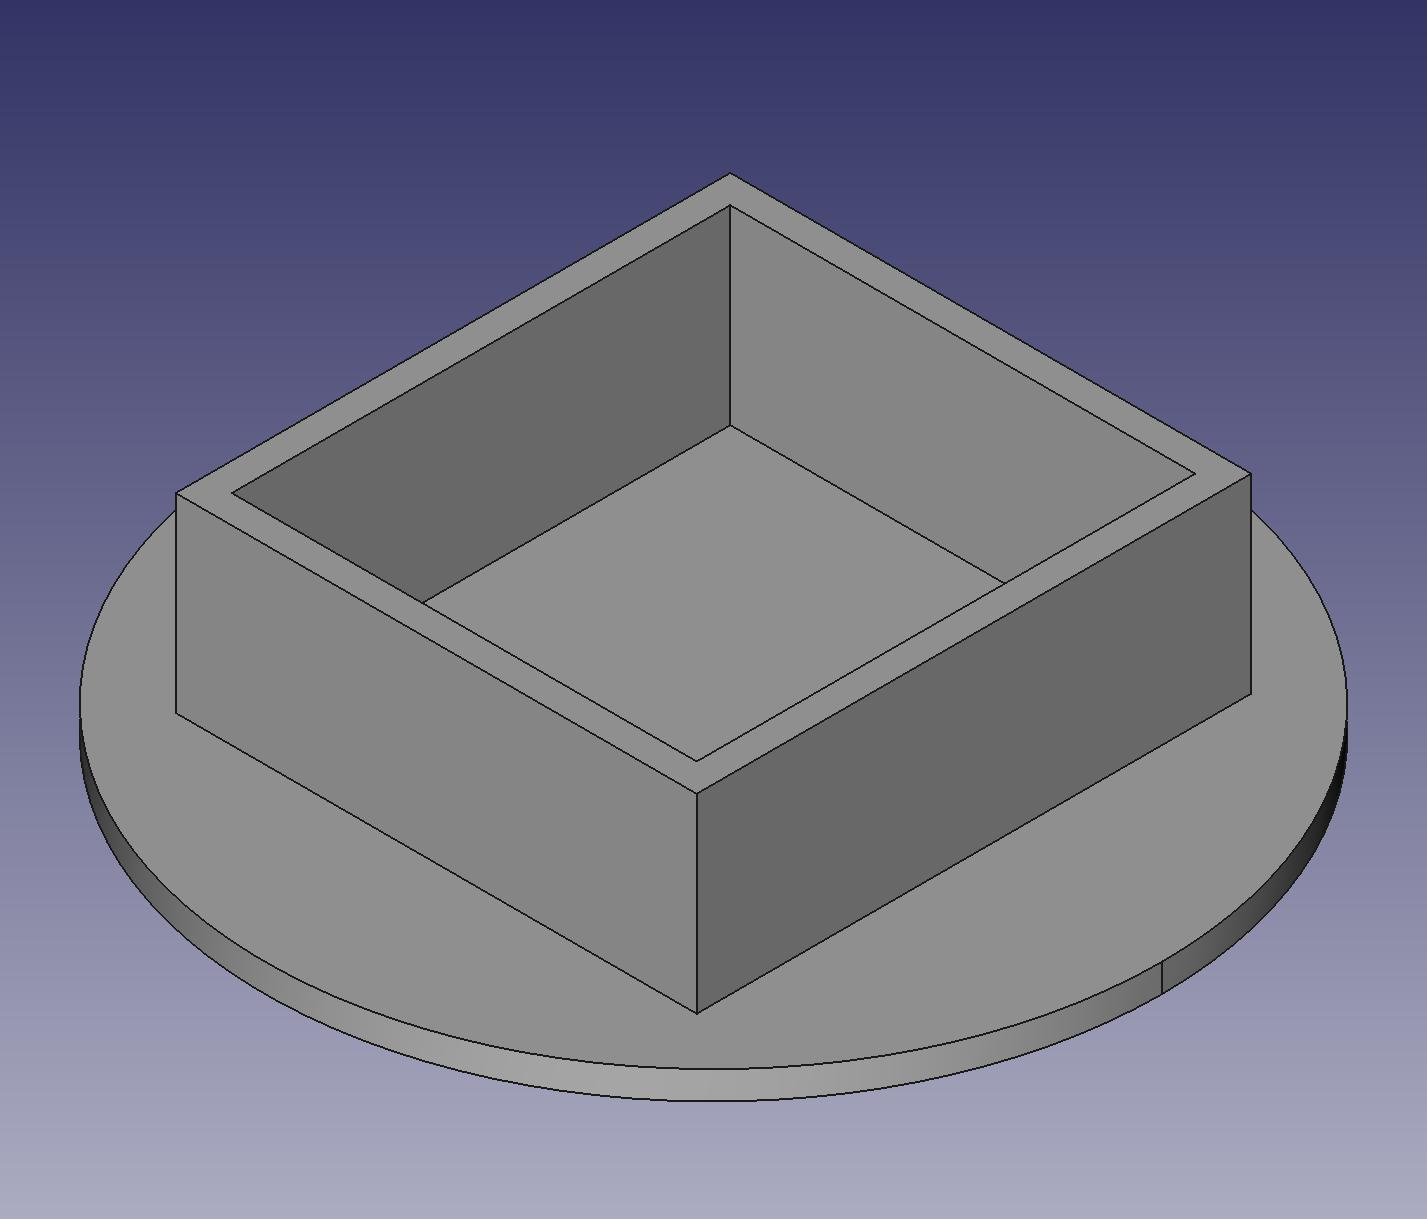
\includegraphics[width=0.45\textwidth]{partbin.jpg}
   \caption{3D sketch of partbin}
\end{figure}


\section{Communication Design}
The communications system needs to follow the following requirements:
\begin{itemize}
	\item Use of XAPI and XBee hardware
	\item Define required TUN packets for communication system 
	\begin{itemize}
		\item Manual drone instructions
		\item Settings and status
		\item ACK
		\item Heartbeat
		\item Override
		\item Mission plan protocol types
	\end{itemize}
\end{itemize}

The following sections will break the communication system down into its several components and detail their design.

	\subsection{Communication Overview}
	Our communications system, as depicted in the graphic below, requires two-way communication between the computer (including the attached Arduino) and the Arduino located on the drone. This system will take an instruction created on the computer, send it over serial to the connected Arduino, pass it to XAPI, XAPI will ship it over XBee to the Arduino on the drone, and a flight control service will execute the instruction. 
	
	\begin{figure}[h!]

  		\centering
    	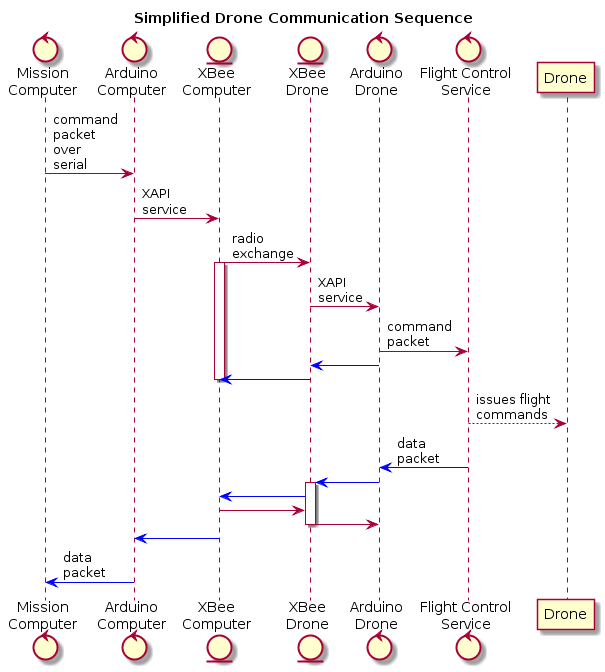
\includegraphics[width=0.5\textwidth]{droneControlSequence.png}
   		\caption{Overview of communications system}
	\end{figure}
	
	\subsection{Hardware Components}
	Our current communications requires the following hardware components:
	\begin{itemize}
		\item Arduino Mega 2560
		\item XBee modules
		\item LCD Shields (for development and debugging)
		\item Serial add-on for Arduino
		\item A computer running Windows to communicate with base Arduino (Workstation needs to be able to run C\# programs)
	\end{itemize}
	
	\subsection{XAPI}
	To satisfy one of our major requirements, we run the XAPI on each Arduino in the communications system. 
	
	XAPI is, put simply, a micro-controller service manager that communicates, both internally and externally, using TUN packets. When communicating externally, the XAPI ships the TUN packet using the XBee hardware by embedding the TUN packet in a XBee packet.
	
	Each service available with the API use XAPI to communicate, using XAPI as the core that each service "latches" to. For instance, if a chat service wanted to display a message on a attached LCD screen, the following steps would be carried out:
	\begin{enumerate}
		\item Chat service creates a LOCAL\_ LCD TUN packet
		\item Chat service passes the newly created packet to the XAPI core
		\item XAPI places the packet in its internal packet buffer
		\item The LCD service latch queries XAPI for any packets designated for the LCD service
		\item LCD service grabs LOCAL\_ LCD TUN packet
		\item LCD service processes and displays the packet
	\end{enumerate}
	
To satisfy our project's requirements, we need to design a Flight Control service that will be able to handle any instruction packets and translate them to instructions that can be given to the drone's flight computer. In addition to this, there is a requirement for a Mission Plan service that will store and execute flight plan's designed by the user and sent to the drone.

	\subsection{TUN Packet Types}
	The following is a table of all the TUN packets types that will be required for this design:
	
	\begin{tabular}{l | l | l}
	TUN Type Key & Payload & Use \\
	Internal/External &  & \\
	\hline
	0x50/0x51 & Altitude & Take off and maintain specific altitude \\
	0x52/0x53 & N/A & Land \\ 
	0x54/0x55 & X,Y,Altitude & Go to specific\\
	& & coordinate \\
	0x56/0x57 & MoveDirection,Amount,Metric & Carry out specific move\\  		& & (North/South/East/West) \\
	0x5C/0x5D & Rotation & Rotate specific amount \\
	0x58/0x59 & N/A & Start mission plan upload \\
	0x60/0x61 & X,Y,Altitude & Mission instruction - go to specific\\ & & coordinate \\
	0x62/0x63 & MoveDirection,Amount,Metric & Mission instruction - carry out specific move\\
	& & (North/South/East/West) \\
	0x6A/0x6B &  & Instruction - Land \\  
	0x5A/0x5B & Altitude & Instruction - Take off and maintain \\ 		    & & specific altitude \\
	0x6C/0x6D & X,Y,Altitude & Instruction - Go to  \\
		& & specific coordinate \\
	0x6E/0x6F & Rotation & Instruction - Rotate specific amount \\
	0x64/0x65 & ChecksumValue & End install and check checksum to\\ 	& & validate success \\
	0x66/0x67 & N/A & Stop current mission plan and activate\\
	& & manual control (maintain altitude) \\
	0x68/0x69 & N/A & Stop current mission plan and activate\\
	& & manual control (no longer autonomous) \\
	0x70/0x71 & N/A & Acknowledgment (ACK)\\
	0x72/0x73 & N/A & Acknowledgment of issue (NACK) \\
	0x74/0x75 & InstrumentData & Heartbeat that contains the drone's\\ & & current state \\ 
	0x76/0x77 & Altitude & Set altitude \\
	0x78/0x79 & Speed & Set the never exceed speed \\ 
	0x80/0x81 & Speed & Set never exceed fall speed \\
	0x82/0x83 & Throttle & Set throttle
	
	\end{tabular}
	
	\subsection{Mission Plan Upload Protocol}
	In order for the drone to autonomously carry out a mission plan, the plan must be uploaded from the source computer to the drone's micro-controller. The following is depicts the Mission Plan upload protocol:
	

	\begin{figure}[h!]

  		\centering
    	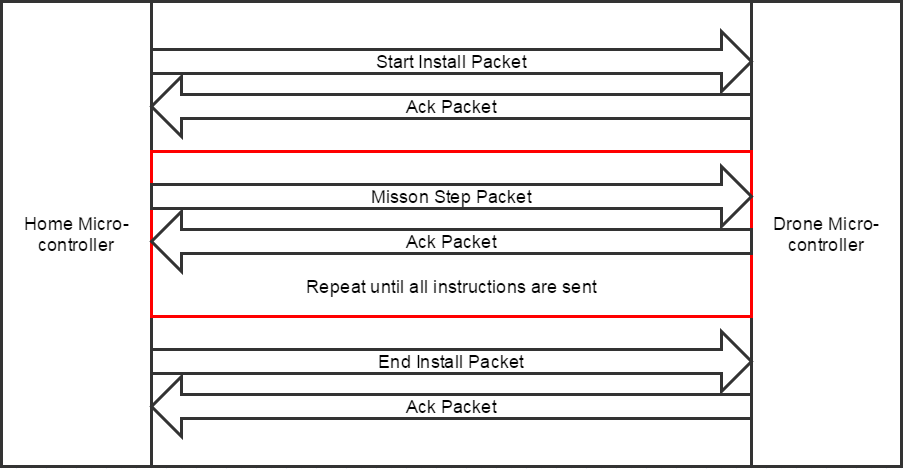
\includegraphics[width=0.75\textwidth]{InstallProcessIdea1.png}
   		\caption{Mission plan upload process}
	\end{figure}
	
	Simply put, an installation packet is used to signal the start of a mission plan upload, each instruction is then sent one at a time, and finally an end installation packet with the checksum of the final mission plan file is sent to the drone. After each of these packets are received by the drone, the drone will send an acknowledgement (ACK) packet. It should be noted that the final ACK packet can be a NACK packet if the checksum received is not the same as the one calculated.

\section{Graphical User Interface Design}
The graphical user interface must satisfy several requirements:
\begin{enumerate}
	\item Must be user-friendly
	\item Allow 3-dimensional mission planning
	\item Allow upload of flight plan to drone
	\item Allow manual override
\end{enumerate}

Given these requirements we were able to design a general design for the graphical user interface (GUI), as shown below. This GUI is split into several sections that convey different information, that in some cases can be adjusted. 

We have a flight control section (light-blue) that shows the status of the drone components and allows the user to "zero out" each component or take manual control. The status information section (yellow) shows different readings from the drone's on-board instruments. The flight planning system (light-red) will be where the user can develop a flight plan to be uploaded to the drone (note that this functionality is still under design and may end up being a separate window that needs to be opened up). The final section is the communications terminal (light-green) that displays all packets sent and received on the Arduino attached to the source computer. This communications terminal will allow the user to see that the drone is still connected and will allow for easy communications debugging.

	\begin{figure}[h!]

  		\centering
    	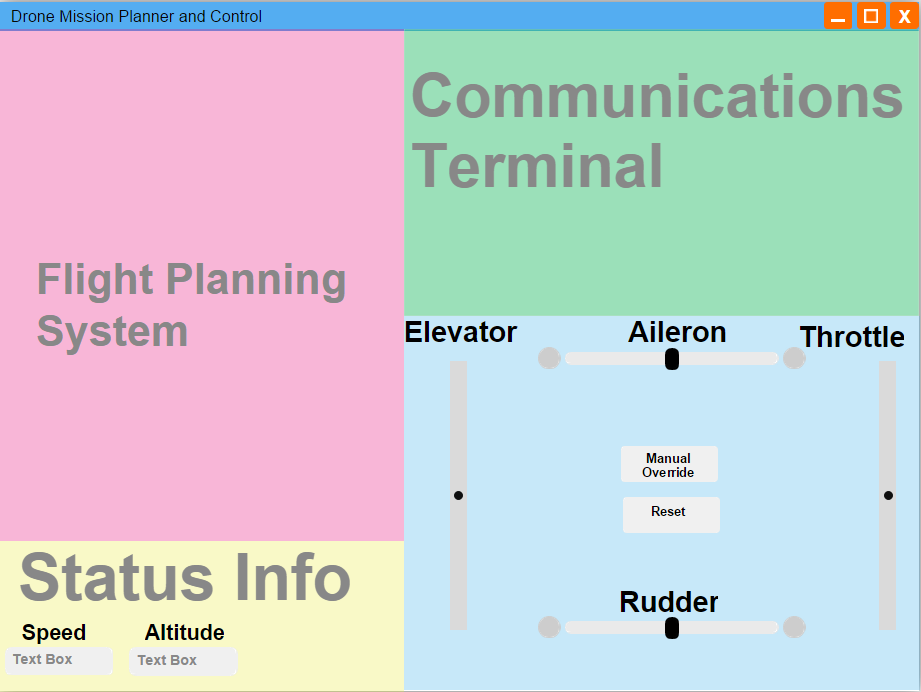
\includegraphics[width=0.75\textwidth]{guiMockup.png}
   		\caption{Graphical user interface mock-up design}
	\end{figure}


\end{document}